\documentclass[12pt]{article}

% packages :
\usepackage[utf8x]{inputenc}
\usepackage[T1]{fontenc}
%\usepackage[francais]{babel}
%
\usepackage{graphicx} % images
\usepackage{float}
\usepackage{placeins}
\usepackage{multirow}
\usepackage{wrapfig}
\usepackage{array}

% to draw circuits
\usepackage{siunitx}
\usepackage{tikz}
\usetikzlibrary{calc}
\usetikzlibrary{decorations.pathmorphing,patterns}

\usepackage[top=2cm, bottom=2cm, left=2.5cm, right=2.5cm]{geometry}


% maths :
\usepackage{amsthm}
\usepackage{amsmath}
\usepackage{amssymb}
\usepackage{mathrsfs}

\usepackage{braket}

\begin{document}

\begin{center}
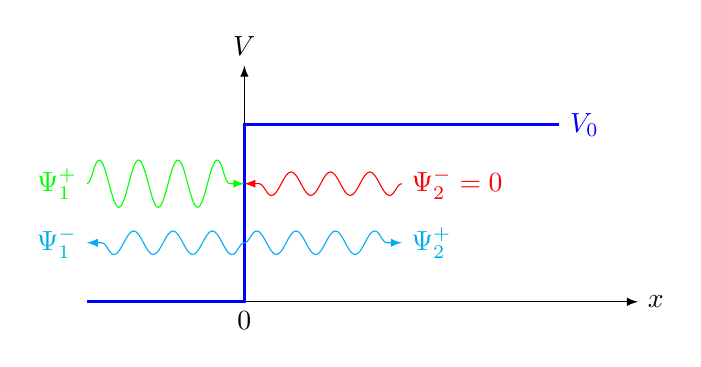
\begin{tikzpicture}
\draw[latex-] (7,0) node[right]{$x$} -- (0,0);
\draw[-latex] (2,0) node[below]{$0$} -- +(0, 3) node[above]{$V$};
\draw[very thick,blue] (0,0) -- (2,0) -- (2,2.25) -- +(4,0) node[right]{$V_0$};
\draw[decoration={segment length=5mm, amplitude=3mm,snake},decorate,-latex,green] (0,1.5) node[left]{$\Psi_1^{+}$} -- +(2,0);
\draw[decoration={segment length=5mm, amplitude=1.5mm,snake},decorate,-latex,cyan] (2,0.75)  -- +(-2,0)node[left]{$\Psi_{1}^-$};
\draw[decoration={segment length=5mm, amplitude=1.5mm,snake},decorate,-latex,cyan] (2,.75) -- +(2,0) node[right]{$\Psi_{2}^+$} ;
\draw[decoration={segment length=5mm, amplitude=1.5mm,snake},decorate,-latex,red] (4,1.5)node[right]{$\Psi_{2}^-=0$}  -- +(-2,0);
\end{tikzpicture}
\end{center}

\begin{center}
    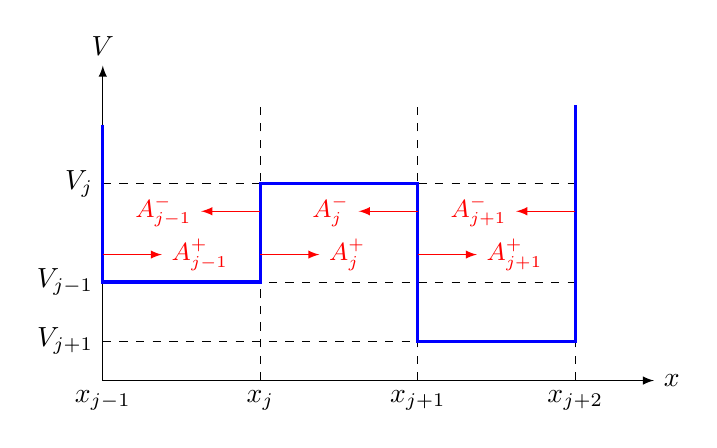
\begin{tikzpicture}
    \draw[-latex] (0,-.25) node[below]{$x_{j-1}$} -- +(7,0) node[right]{$x$} ;
    \draw[-latex] (0,-.25) -- +(0, 4) node[above]{$V$};
    \draw[dashed] (2,-.25) node[below]{$x_j$}-- +(0,3.5);
    \draw[dashed] (4,-.25) node[below]{$x_{j+1}$}-- +(0,3.5);
    \draw[dashed] (6,-.25) node[below]{$x_{j+2}$}-- +(0,3.5);
    \draw[dashed] (0,1)  node[left]{$V_{j-1}$} -- +(6,0);
    \draw[dashed] (0,2.25)  node[left]{$V_{j}$} -- +(6,0);
    \draw[dashed] (0,.25)  node[left]{$V_{j+1}$} -- +(6,0);
    \draw[very thick,blue] (0,3) -- (0,1) -- (2,1) -- (2,2.25) -- ++(2,0) -- ++(0,-2) -- ++ (2,0) -- ++(0,3);
    \draw[-latex,red] (0,1.35) -- +(.75,0) node[right]{\small $A^+_{j-1}$};
    \draw[-latex,red] (2,1.9) -- +(-.75,0) node[left]{\small $A^-_{j-1}$};
    \draw[-latex,red] (2,1.35) -- +(.75,0) node[right]{\small $A^+_{j}$};
    \draw[-latex,red] (4,1.9) -- +(-.75,0) node[left]{\small $A^-_{j}$};
    \draw[-latex,red] (4,1.35) -- +(.75,0) node[right]{\small $A^+_{j+1}$};
    \draw[-latex,red] (6,1.9) -- +(-.75,0) node[left]{\small $A^-_{j+1}$};
    \end{tikzpicture}
\end{center}


\begin{center}
    \begin{tikzpicture}
    \draw[-latex] (0,-.25) -- +(7,0) node[right]{$x$} ;
    \draw[-latex] (0,-.25) -- +(0, 4) node[above]{$V$};
    \draw[dashed] (2,-.25) node[below]{$0$}-- +(0,3.5);
    \draw[dashed] (4,-.25) node[below]{$a$}-- +(0,3.5);
    \draw[dashed] (0,2.25)  node[left]{$V_0$} -- +(6,0);
    \draw[dashed] (0,.25)  node[left]{$0$} -- +(6,0);
    \draw[very thick,blue] (0,.25) -- (2,.25) -- ++(0,2) -- ++(2,0) -- ++(0,-2) -- ++ (2,0);
    \draw[-latex,red] (0,1.35) -- +(.75,0) node[right]{\small $A^+_{0}$};
    \draw[-latex,red] (2,1.9) -- +(-.75,0) node[left]{\small $A^-_{0}$};
    \draw[-latex,red] (2,1.35) -- +(.75,0) node[right]{\small $A^+_{1}$};
    \draw[-latex,red] (4,1.9) -- +(-.75,0) node[left]{\small $A^-_{1}$};
    \draw[-latex,red] (4,1.35) -- +(.75,0) node[right]{\small $A^+_{2}$};
    \end{tikzpicture}
\end{center}

\begin{center}
    \begin{tikzpicture}
    \draw[-latex] (0,-.25) -- +(7,0) node[right]{$x$} ;
    \draw[-latex] (0,-.25) -- +(0, 4) node[above]{$V$};
        \draw[dashed] (2,-.25) node[below]{$a$}-- +(0,3.5);
    \draw[dashed] (4,-.25) node[below]{$b$}-- +(0,3.5);
    \draw[dashed] (0,2.25)  node[left]{$V_2$} -- +(6,0);
    \draw[dashed] (0,.25)  node[left]{$V_1$} -- +(6,0);
    \draw[dashed] (0,1.25)  node[left]{$(V_2-V_1)/2$} -- +(6,0);
    \draw[thick,red,dashed] (2,2.25) -- ++(1,0) -- ++(0,-1) -- ++(1,0) -- +(0,-1);
    \draw[very thick,blue] (0,.25) -- (2,.25) -- ++(0,2) -- ++(2,-2) -- ++ (2,0);
    \end{tikzpicture}
\end{center}

\end{document}